%=============================================================================
% Résumé Optimization Using Generative AI — two-column draft
%
% Compiles with IEEEtran (Overleaf: "IEEE Conference" template, or upload this
% file and select pdfLaTeX). If IEEEtran.cls is unavailable, swap the first
% line for \documentclass[twocolumn,10pt]{article} and delete \IEEEpeerreviewmaketitle.
%=============================================================================
\documentclass[conference]{IEEEtran}

\usepackage[utf8]{inputenc}
\usepackage[T1]{fontenc}
\usepackage{amsmath,amssymb}
\usepackage{booktabs}
\usepackage{graphicx}
\usepackage{tikz}
\usetikzlibrary{arrows.meta, positioning, fit, backgrounds}
\usepackage{url}
\usepackage{balance}

\begin{document}

\title{Résumé Optimization Using Generative AI:\\
A Provenance-Verified Rewrite Gate}

\author{\IEEEauthorblockN{[Author Name]}
\IEEEauthorblockA{[Department]\\
[Institution]\\
[email@domain]}}

\maketitle

\begin{abstract}
Generative language models make résumé tailoring trivial to prototype and
dangerous to deploy: a rewriter that invents a skill, an employer, or a metric
produces a document that scores better and misrepresents the candidate. We argue
this is a structural problem rather than a prompt-engineering one, because the
optimization objective and the failure mode point in the same direction --- an
invented keyword is precisely the keyword the job description asked for, so any
match-based metric ranks a fabricating system above an honest one. We present a
résumé optimization pipeline built on a \emph{provenance chain}: every value
extracted from a source document carries a stable identifier pointing at the
exact span supporting it, and that identifier survives through matching,
scoring, and rewriting. A deterministic, LLM-free \emph{verification gate} then
checks every value the rewriter proposes against that chain and deletes whatever
cannot be traced. On 30 résumé/job-description pairs, prompt grounding alone
shipped 40 unsourced claims, affecting 33\% of documents; with the gate enabled,
zero unsourced claims reached the output, reproduced on a second, independently
hosted model. We report the gate's cost as well as its benefit, and argue the
central finding is not the zero --- true by construction --- but the measured
inadequacy of prompt grounding that motivates it.
\end{abstract}

\begin{IEEEkeywords}
generative AI, résumé optimization, hallucination mitigation, provenance,
applicant tracking systems, verified generation.
\end{IEEEkeywords}

\IEEEpeerreviewmaketitle

%-----------------------------------------------------------------------------
\section{Introduction}

Résumé optimization --- taking a candidate's résumé and a target job
description, producing a tailored version plus a predicted match score --- is
now routinely built as a generative-AI pipeline. Document parsing has largely
shifted from named-entity recognition to LLM extraction under
schema-constrained decoding \cite{docling,outlines,vllm}, which buys reliability
on the \emph{structure} of the output.

It does not buy reliability on the \emph{content}. A rewriting stage asked to
``tailor'' a résumé toward a set of requirements is exactly the setting in which
language models fabricate: invented metrics, employers that never existed,
skills the candidate never claimed. In hiring this is not cosmetic. A résumé
fabricated by the tool the candidate trusted misrepresents them to an employer,
with consequences they did not choose and may not be aware of.

The core difficulty is that the obvious objective is adversarial to
truthfulness. If a résumé lacks \emph{Kubernetes} and the posting demands it,
the single most effective way to raise any keyword- or embedding-based match
score is to add \emph{Kubernetes}. \textbf{Optimizing for match score actively
rewards fabrication.} An evaluation measuring only score improvement therefore
cannot distinguish a good system from a dishonest one, and a system tuned on
such a metric is being trained toward the failure it should avoid.

We take the position that truthfulness has a specific, checkable shape rather
than being a prompt-engineering aspiration. Concretely: \emph{every hard-content
token in a rewritten résumé --- skill, tool, organization, number, date --- must
trace to at least one span in the original document that supports it}. We call
this the \textbf{provenance invariant}. A rewrite that cannot demonstrate the
invariant for a value does not ship that value.

\subsection{Contributions}
\begin{itemize}
  \item \textbf{C1.} A continuous provenance chain established at ingestion and
    threaded unbroken into every downstream representation of the résumé.
  \item \textbf{C2.} A match score calibrated against a real, rule-based ATS
    engine rather than reported as a raw embedding-similarity proxy.
  \item \textbf{C3.} A deterministic, LLM-free rewrite gate that rejects
    unsupported values before they ship, reporting a fabrication rate as a
    first-class metric rather than assuming it away.
\end{itemize}

%-----------------------------------------------------------------------------
\section{Related Work}

\textbf{Layout-aware extraction.} Digital-native PDF parsers scramble reading
order on multi-column layouts, the largest reported cause of downstream
extraction error. Docling \cite{docling} unifies PDF, DOCX and image inputs into
a single representation preserving reading order and table structure.
Specialised layout models \cite{layoutlm} and OCR-free document transformers
\cite{donut} are a heavier alternative better suited to bespoke extractors than
to systems built atop general-purpose LLMs.

\textbf{Constrained decoding.} Three reliability tiers are commonly
distinguished: prompt-only JSON requests (unreliable), function-calling or JSON
mode (syntactically valid but not schema-guaranteed), and constrained decoding,
which masks invalid tokens during generation so output cannot violate the
schema. Outlines \cite{outlines} and vLLM \cite{vllm} implement this for
self-hosted models; hosted APIs expose equivalent mechanisms. Crucially,
constrained decoding guarantees output \emph{shape}, never output \emph{truth}
--- a distinction central to this work.

\textbf{ATS matching.} Applicant tracking systems are typically a parser stage
followed by a matcher combining keyword coverage with semantic similarity
\cite{sbert}. Systems reporting a match score from raw cosine similarity
conflate two different quantities: how similar two embeddings are, and how an
actual ATS would score the pair. We calibrate against the latter directly.

\textbf{Fabrication in LLM rewriting.} Résumé rewriters lacking an explicit
truthfulness mechanism exhibit documented failure modes: invented metrics,
fabricated employers and titles, temporal fabrication, and cross-domain
contamination between unrelated sections. Prompt grounding measurably reduces
but does not eliminate this, as our gate-OFF measurements confirm
(Section~\ref{sec:results}). This is our central argument for a deterministic
verification gate rather than a stronger prompt.

%-----------------------------------------------------------------------------
\section{System Architecture}

\begin{figure}[t]
\centering
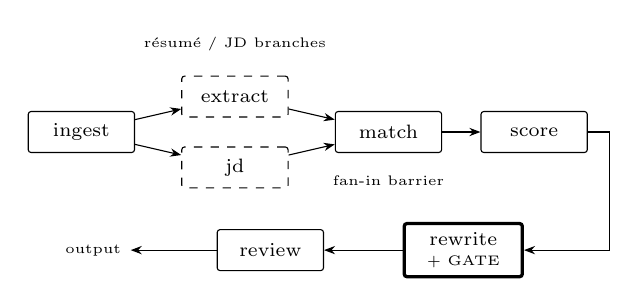
\begin{tikzpicture}[
  font=\scriptsize,
  det/.style={draw, rounded corners=1pt, minimum width=1.35cm,
              minimum height=0.52cm, align=center},
  sto/.style={draw, dashed, rounded corners=1pt, minimum width=1.35cm,
              minimum height=0.52cm, align=center},
  gate/.style={draw, very thick, rounded corners=1pt, minimum width=1.5cm,
               minimum height=0.52cm, align=center},
  arr/.style={-{Stealth[length=1.4mm]}, thin}
]
\node[det] (ing) at (0,0) {ingest};
\node[sto] (ext) at (1.95,0.45) {extract};
\node[sto] (jd)  at (1.95,-0.45) {jd};
\node[det] (mat) at (3.9,0) {match};
\node[det] (sco) at (5.75,0) {score};

\node[gate] (rew) at (4.85,-1.5) {rewrite\\[-1pt]\tiny + GATE};
\node[det]  (rev) at (2.4,-1.5) {review};
\node       (out) at (0.15,-1.5) {\tiny output};

\draw[arr] (ing) -- (ext);
\draw[arr] (ing) -- (jd);
\draw[arr] (ext) -- (mat);
\draw[arr] (jd)  -- (mat);
\draw[arr] (mat) -- (sco);
\draw[arr] (sco.east) -- ++(0.28,0) |- (rew.east);
\draw[arr] (rew) -- (rev);
\draw[arr] (rev) -- (out);

\node[align=center] at (1.95,1.12) {\tiny résumé / JD branches};
\node[align=center] at (3.9,-0.62) {\tiny fan-in barrier};
\end{tikzpicture}
\caption{The seven-node pipeline. Solid boxes are deterministic; dashed boxes
are stochastic (LLM) stages; the gate is drawn bold. Résumé parsing and
job-description analysis are independent and overlap in wall-clock time;
\texttt{match} is a \emph{deferred} fan-in barrier rather than a
first-input-wins trigger, so it never observes a partially populated state.
Every stochastic stage is immediately followed by a deterministic stage that
checks it.}
\label{fig:pipeline}
\end{figure}

The system is a seven-node directed graph \cite{langgraph} with two parallel
branches fanning in at matching (Fig.~\ref{fig:pipeline}). The architectural
principle is visible in the figure: \emph{no stochastic stage is the last word
on anything factual}. Each is followed by a deterministic stage that verifies
its output.

\subsection{Models Used and Why}

\textbf{Ingestion: Docling.} Chosen for layout-aware conversion because reading
order on multi-column résumés is the dominant source of extraction error, and
because it emits per-item geometry (page, bounding box, character offsets) ---
which is what makes a provenance chain constructible at all. A plain text
extractor would foreclose C1 entirely.

\textbf{Extraction, JD analysis, rewriting:
\texttt{gemini-3.1-flash-lite}.} A hosted model exposing genuine
\texttt{responseSchema} constrained decoding, so malformed structured output is
prevented at the decoding level rather than repaired afterward. Every result is
cross-checked on a locally hosted \texttt{qwen2.5:14b} via Ollama
\cite{ollama,qwen} to establish that the safety guarantee is not an artifact of
one vendor's generation style. The rewriter runs at temperature 0.6 ---
deliberately creative, because the gate is what makes creativity safe;
extraction runs at temperature 0 for reproducibility.

\textbf{Semantic matching: \texttt{all-mpnet-base-v2}.} Selected as the
quality-tier model of the Sentence-BERT family \cite{sbert} on task-shape
grounds: comparing a short requirement against short résumé strings is
\emph{symmetric} short-text similarity, which \texttt{all-*} models target,
whereas \texttt{multi-qa-*} variants are trained for asymmetric
query--document retrieval. Throughput is irrelevant at this position --- the
embedder processes tens of strings per request behind LLM calls costing seconds
--- so the faster, weaker MiniLM variants offer no benefit. Embeddings are
normalized, reducing cosine similarity to a dot product.

\textbf{Calibration: Ridge regression.} With 199 pairs and five features, a
higher-capacity model would overfit; linear coefficients also remain
inspectable, which matters for a pipeline whose premise is auditability.
Terminating an auditable chain in an uninterpretable scorer would be
self-defeating.

\subsection{Provenance Chain (C1)}

At ingestion each text item becomes a \texttt{SourceSpan} recording its
document, character offsets into the exported markdown, page, bounding box, and
raw text. Every value-bearing field produced by extraction carries a sibling
provenance list of supporting span identifiers. This is attached \emph{during}
extraction rather than reconstructed afterward, and is what the gate later
checks against. Span resolution is intentionally fuzzy: exact matching would
reject truthful content over invisible formatting noise such as a bullet glyph
or a line break mid-phrase.

\subsection{Calibrated Scoring (C2)}

The matcher emits a five-dimensional feature vector --- keyword coverage,
semantic similarity, fuzzy coverage, must-have coverage, nice-to-have coverage
--- computed over the whole résumé rather than the skills list alone, since
requirement evidence usually sits in an experience bullet. Rather than reporting
a hand-weighted function of this vector, a Ridge regression is fit against the
output of a self-hostable rule-based ATS simulator \cite{atsscreener}.

The regression target is the simulator's \emph{job-description-dependent}
dimension only. Its composite score is dominated by résumé-intrinsic signals
(formatting, section completeness) that do not vary with the posting;
calibrating against the composite yields a target our match features correlate
\emph{negatively} with, because we would be predicting résumé quality rather
than fit.

%-----------------------------------------------------------------------------
\section{The Verification Gate (C3)}

The gate is this work's central mechanism. Three properties define it:

\begin{itemize}
  \item \textbf{Subtractive.} It can only delete, never rewrite, so it cannot
    itself introduce content.
  \item \textbf{Deterministic.} Pure string matching and regular expressions
    --- no model, no randomness. The same inputs always yield the same verdict,
    which is what makes the reported fabrication rate a reproducible measurement
    rather than one model's opinion of another.
  \item \textbf{Post-hoc.} It inspects finished text, so it is independent of
    which model produced it --- the basis for the cross-backend result.
\end{itemize}

The rewriter is prompted with the source résumé as sole source of truth and
instructed to reorder, rephrase and emphasise but never invent, and to leave a
requirement honestly unsatisfied rather than fabricate coverage.
\textbf{This prompt is deliberately not the safety mechanism};
Section~\ref{sec:results} measures how often it fails.

The gate distinguishes two content classes, which fail differently.

\subsection{Short Factual Values}

Skills, tools, titles, employers, certifications. Two conditions apply in
sequence. First, candidate evidence is located by fuzzy substring search over
all spans, tolerant enough to survive formatting noise. Second, and critically,
\emph{locating a span is necessary but not sufficient}: because substring
scoring returns the best-matching window, a span reading \texttt{Engineer}
scores a perfect match against the fabricated promotion \texttt{Staff
Engineer}. Every content word of an added value must therefore appear in the
supporting span, or the unmatched words are unsourced claims. Function words are
exempt, since requiring provenance for them would reject truthful rewordings.

\subsection{Bullets}

Rephrasing prose is legitimate --- indeed it is the rewriter's job --- so exact
tests are inappropriate. Bullets are compared whole-string against source
bullets using order-independent token-set overlap. Similarity alone is
insufficient, however: a long invention recycling the source's vocabulary scores
well, as in \emph{``Led a team of 40 Teradata engineers.''} A bullet is
therefore accepted only if it (i) closely tracks some source bullet
\textbf{and} (ii) introduces no unsourced \emph{hard-content token}, where hard
content means capitalised terms mid-sentence, all-caps acronyms, and digit runs.
Prose may change freely; facts may not appear from nowhere. Inflections are
collapsed by a deliberately crude stemmer, so ordinary rewording does not read
as a new claim.

\subsection{Threshold Derivation}

\begin{table}[t]
\centering
\caption{Gate thresholds. All are string-edit ratios, not cosine similarities.}
\label{tab:thresholds}
\begin{tabular}{@{}llp{3.6cm}@{}}
\toprule
Test & Value & Basis \\
\midrule
Bullet similarity & 60 & Measured: rephrasings score 68--87, inventions 37--42; 60 sits in the empty band \\
Word support & 88 & Conventional high-confidence cut, loosened for inflection \\
Span resolution & 90 & Conventional; treated as necessary-not-sufficient \\
\bottomrule
\end{tabular}
\end{table}

The bullet threshold (Table~\ref{tab:thresholds}) was measured rather than
chosen. On corpus rewrites, genuine rephrasings scored 68--87 and inventions
37--42, leaving an empty band between the classes; a threshold of 90 rejected
\emph{every} genuine rephrasing. Notably none of the gate's thresholds are
cosine similarities --- the gate is deliberately embedding-free, since
determinism is what makes its output a measurement.

\subsection{Independent Re-check}

A final node re-verifies the \emph{shipped} résumé from scratch against the
provenance map, duplicating the gate deliberately. If it fires, the gate leaked.
It reports the violation rather than raising, so a leak is surfaced and logged
rather than silently swallowed.

%-----------------------------------------------------------------------------
\section{Results}
\label{sec:results}

\begin{table}[t]
\centering
\caption{Fabrication gate, 30 corpus-backed pairs. ``Gate OFF'' is the
rewriter's raw output under prompt grounding alone.}
\label{tab:gate}
\begin{tabular}{@{}lcccc@{}}
\toprule
Rewriter backend & Pairs & OFF & ON & Docs affected \\
\midrule
\texttt{gemini-3.1-flash-lite} & 30/30 & 40 & \textbf{0} & 10/30 \\
\texttt{qwen2.5:14b} (local)   & 30/30 & 31 & \textbf{0} & 14/30 \\
\bottomrule
\end{tabular}
\end{table}

\begin{table}[t]
\centering
\caption{Extraction quality and calibration, primary backend.}
\label{tab:quality}
\begin{tabular}{@{}lc@{}}
\toprule
Metric & Value \\
\midrule
Skills F1 (public annotated, $n{=}143$) & 0.753 \\
Job title / institution F1 & 0.935 / 0.917 \\
Provenance-attachment accuracy & 0.874 \\
Calibrated MAE / Spearman $\rho$ & 3.25 / 0.333 \\
Cosine baseline MAE / $\rho$ & 27.58 / 0.229 \\
\bottomrule
\end{tabular}
\end{table}

Expressed as accuracy (Table~\ref{tab:gate}): with the gate off, 66.7\% of
documents shipped completely clean and 44\% of individual proposed edits (40 of
72) were unsourced. With the gate on, those become 100\% and 0\%. The 32
supported edits still shipped --- the gate removed the unsupported subset rather
than suppressing rewriting.

\textbf{Ablation.} Replacing span-resolved provenance with the cheaper
substitute a provenance-free system would use --- a case-insensitive substring
search anywhere in the source text --- catches 36 of 40 rejections but
\textbf{misses 4}: additions appearing somewhere in the document yet unsupported
where the rewriter used them. Those four are the measured value of resolving to
an actual span rather than checking bag-of-words presence.

\textbf{Interpretation.} Gate-ON $=0$ is true \emph{by construction} and is not
offered as an empirical finding; the gate's mechanism is deleting exactly those
claims. The informative result is gate-OFF: an explicitly grounded prompt,
instructing the model that ``an honest gap is the correct output,'' still
shipped 40 unsourced claims. That the guarantee holds identically on a second,
independently hosted model supports the claim that it is a property of the
deterministic gate rather than of one model's generation style.

%-----------------------------------------------------------------------------
\section{Limitations}

The scorer is also the evaluator: improvement is measured against a calibrator
this work fitted, and $\rho = 0.333$ is a modest predictor, not a faithful ATS
simulation. Guarantees inherit provenance accuracy --- at 0.874 roughly one span
in eight is imperfect, so a \emph{truthful} claim whose span was mis-attached is
wrongly rejected; this false-positive rate is the gate's real cost to a user and
is currently unmeasured. The gate checks that nothing is invented but not that
nothing is silently \emph{dropped}; omission is enforced only by prompt
instruction. The benchmark is 30 pairs --- sufficient to demonstrate the effect,
insufficient for a confidence interval on the mean fabrication rate. Semantic
bands used for requirement classification are provisional defaults, never swept
against a labelled match set. Finally, the hard-token heuristic treats Latin
capitalisation as a factual-content signal and would not transfer to a caseless
script.

%-----------------------------------------------------------------------------
\section{Conclusion}

We presented a résumé optimization system in which a provenance identifier space
survives unbroken from ingestion through rewriting, a match score is calibrated
against a real ATS engine rather than an embedding proxy, and a deterministic
gate rejects any value the provenance chain cannot support. The measured result
is that prompt grounding alone is inadequate --- a third of documents shipped at
least one fabricated claim --- while a subtractive, model-independent gate
reduces this to zero on two backends. We further note that truthful tailoring
has a low ceiling, set by what the candidate has actually done, and argue that
making that ceiling visible is more useful than optimizing past it.

\textbf{Future work.} Retained gain, i.e.\ what fraction of ungated score
improvement survives gating; the gate's false-positive rate; an adversarial
rewriter explicitly instructed to evade the gate; and human evaluation against
recruiter judgement.

%-----------------------------------------------------------------------------
\begin{thebibliography}{9}
\balance

\bibitem{docling}
Docling Team, ``Docling: An efficient open-source toolkit for PDF document
conversion,'' 2024.

\bibitem{layoutlm}
Y.~Huang \emph{et al.}, ``LayoutLMv3: Pre-training for document AI with unified
text and image masking,'' \emph{ACM MM}, 2022.

\bibitem{donut}
G.~Kim \emph{et al.}, ``OCR-free document understanding transformer,''
\emph{ECCV}, 2022.

\bibitem{outlines}
B.~T. Willard and R.~Louf, ``Efficient guided generation for large language
models,'' arXiv:2307.09702, 2023.

\bibitem{vllm}
W.~Kwon \emph{et al.}, ``Efficient memory management for large language model
serving with PagedAttention,'' \emph{SOSP}, 2023.

\bibitem{sbert}
N.~Reimers and I.~Gurevych, ``Sentence-BERT: Sentence embeddings using Siamese
BERT-networks,'' arXiv:1908.10084, 2019.

\bibitem{langgraph}
LangChain, ``LangGraph: Building stateful multi-actor applications with LLMs,''
2024.

\bibitem{atsscreener}
``ats-screener: a rule-based applicant tracking system simulator,'' pinned
commit \texttt{4105f77}.

\bibitem{ollama}
Ollama, ``Run large language models locally,'' 2024.

\bibitem{qwen}
Qwen Team, ``Qwen2.5 technical report,'' 2024.

\end{thebibliography}

\end{document}
